%requirement engineering

\section{preparements}
The first task included to figure out, which needed existed in the company. The idea in this project was to do it with the help of
 leading interviews.
First of all we sat together and worked out the main questions, which could help us to finalize the requirements. The questions
mustn't set any direction for the answer. On the one hand they should leave place for a long, subjective answer,, including the
"hidden" informations, which had obviously nothing to do with the main theme, but on the other they should be specific
enough to get as much important information as they can. At least we prepared the guideline in \prettyref{fig:interview1} and 
\prettyref{fig:interview2}

\begin{figure}[!h]
	\centering
	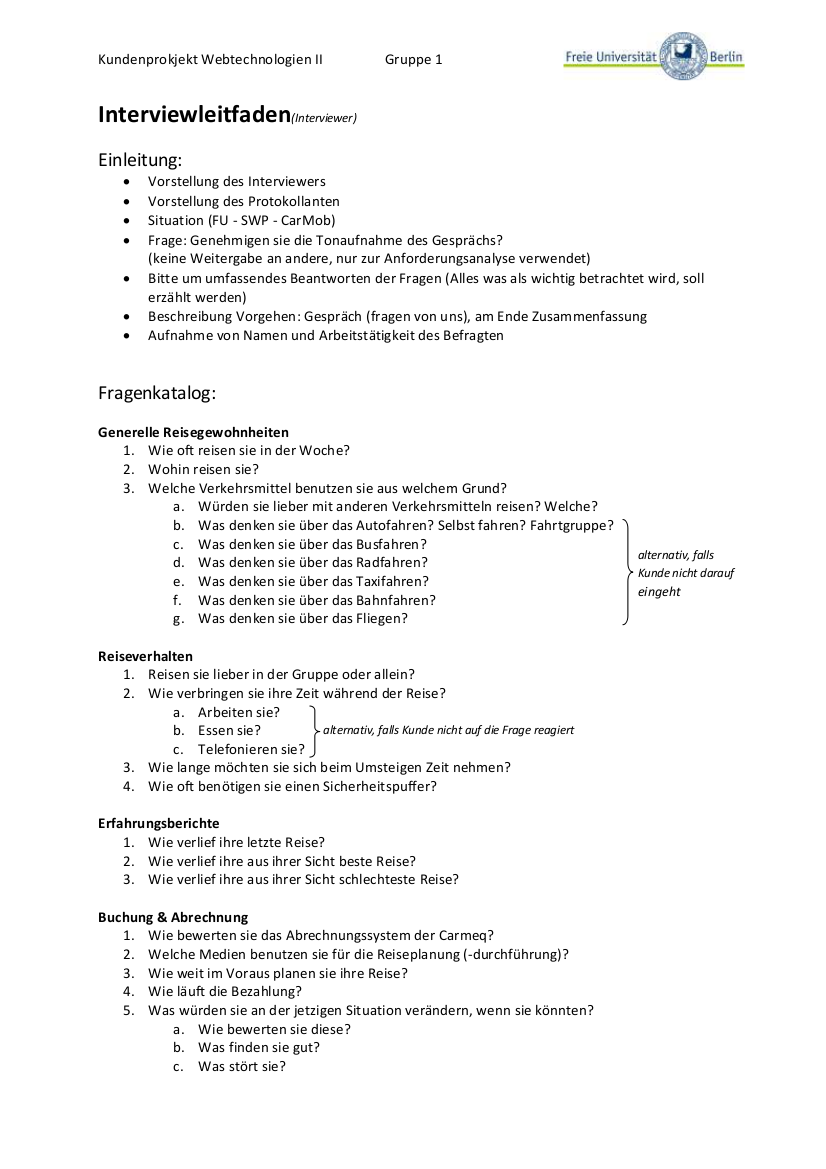
\includegraphics[width=\textwidth, page=1, scale=0.9]{images/Interviewbogen.png}
	\caption{interview sheet 1}
	\label{fig:interview1}
\end{figure}

\clearpage

\begin{figure}[!h]
	\centering
	\includegraphics[width=\textwidth, trim= 0mm 170mm 0mm 30mm,clip, page=2,scale=0.9]{images/Interviewbogen2.png}
	\caption{interview sheet 2}
	\label{fig:interview2}
\end{figure}

\section{implementation}

For leading the interviews we split our team in two group, one of each group records the spoken, the other asked. We tab a total
of four interview, each group got two. After that we tried to reproduce the interviews with the principle of StoryShareCapture and
clustered the needs we find out in main categories. That relieved merging the results and finding similarities, in
\prettyref{fig:mindmap1} you can see our very first try, not 10 minutes after the interviews and in \prettyref{fig:mindmap2}  and
\prettyref{fig:mindmap3} the final digital version.


\begin{figure}[!h]
	\begin{subfigure}[b]{0.29\textwidth}
		\centering
		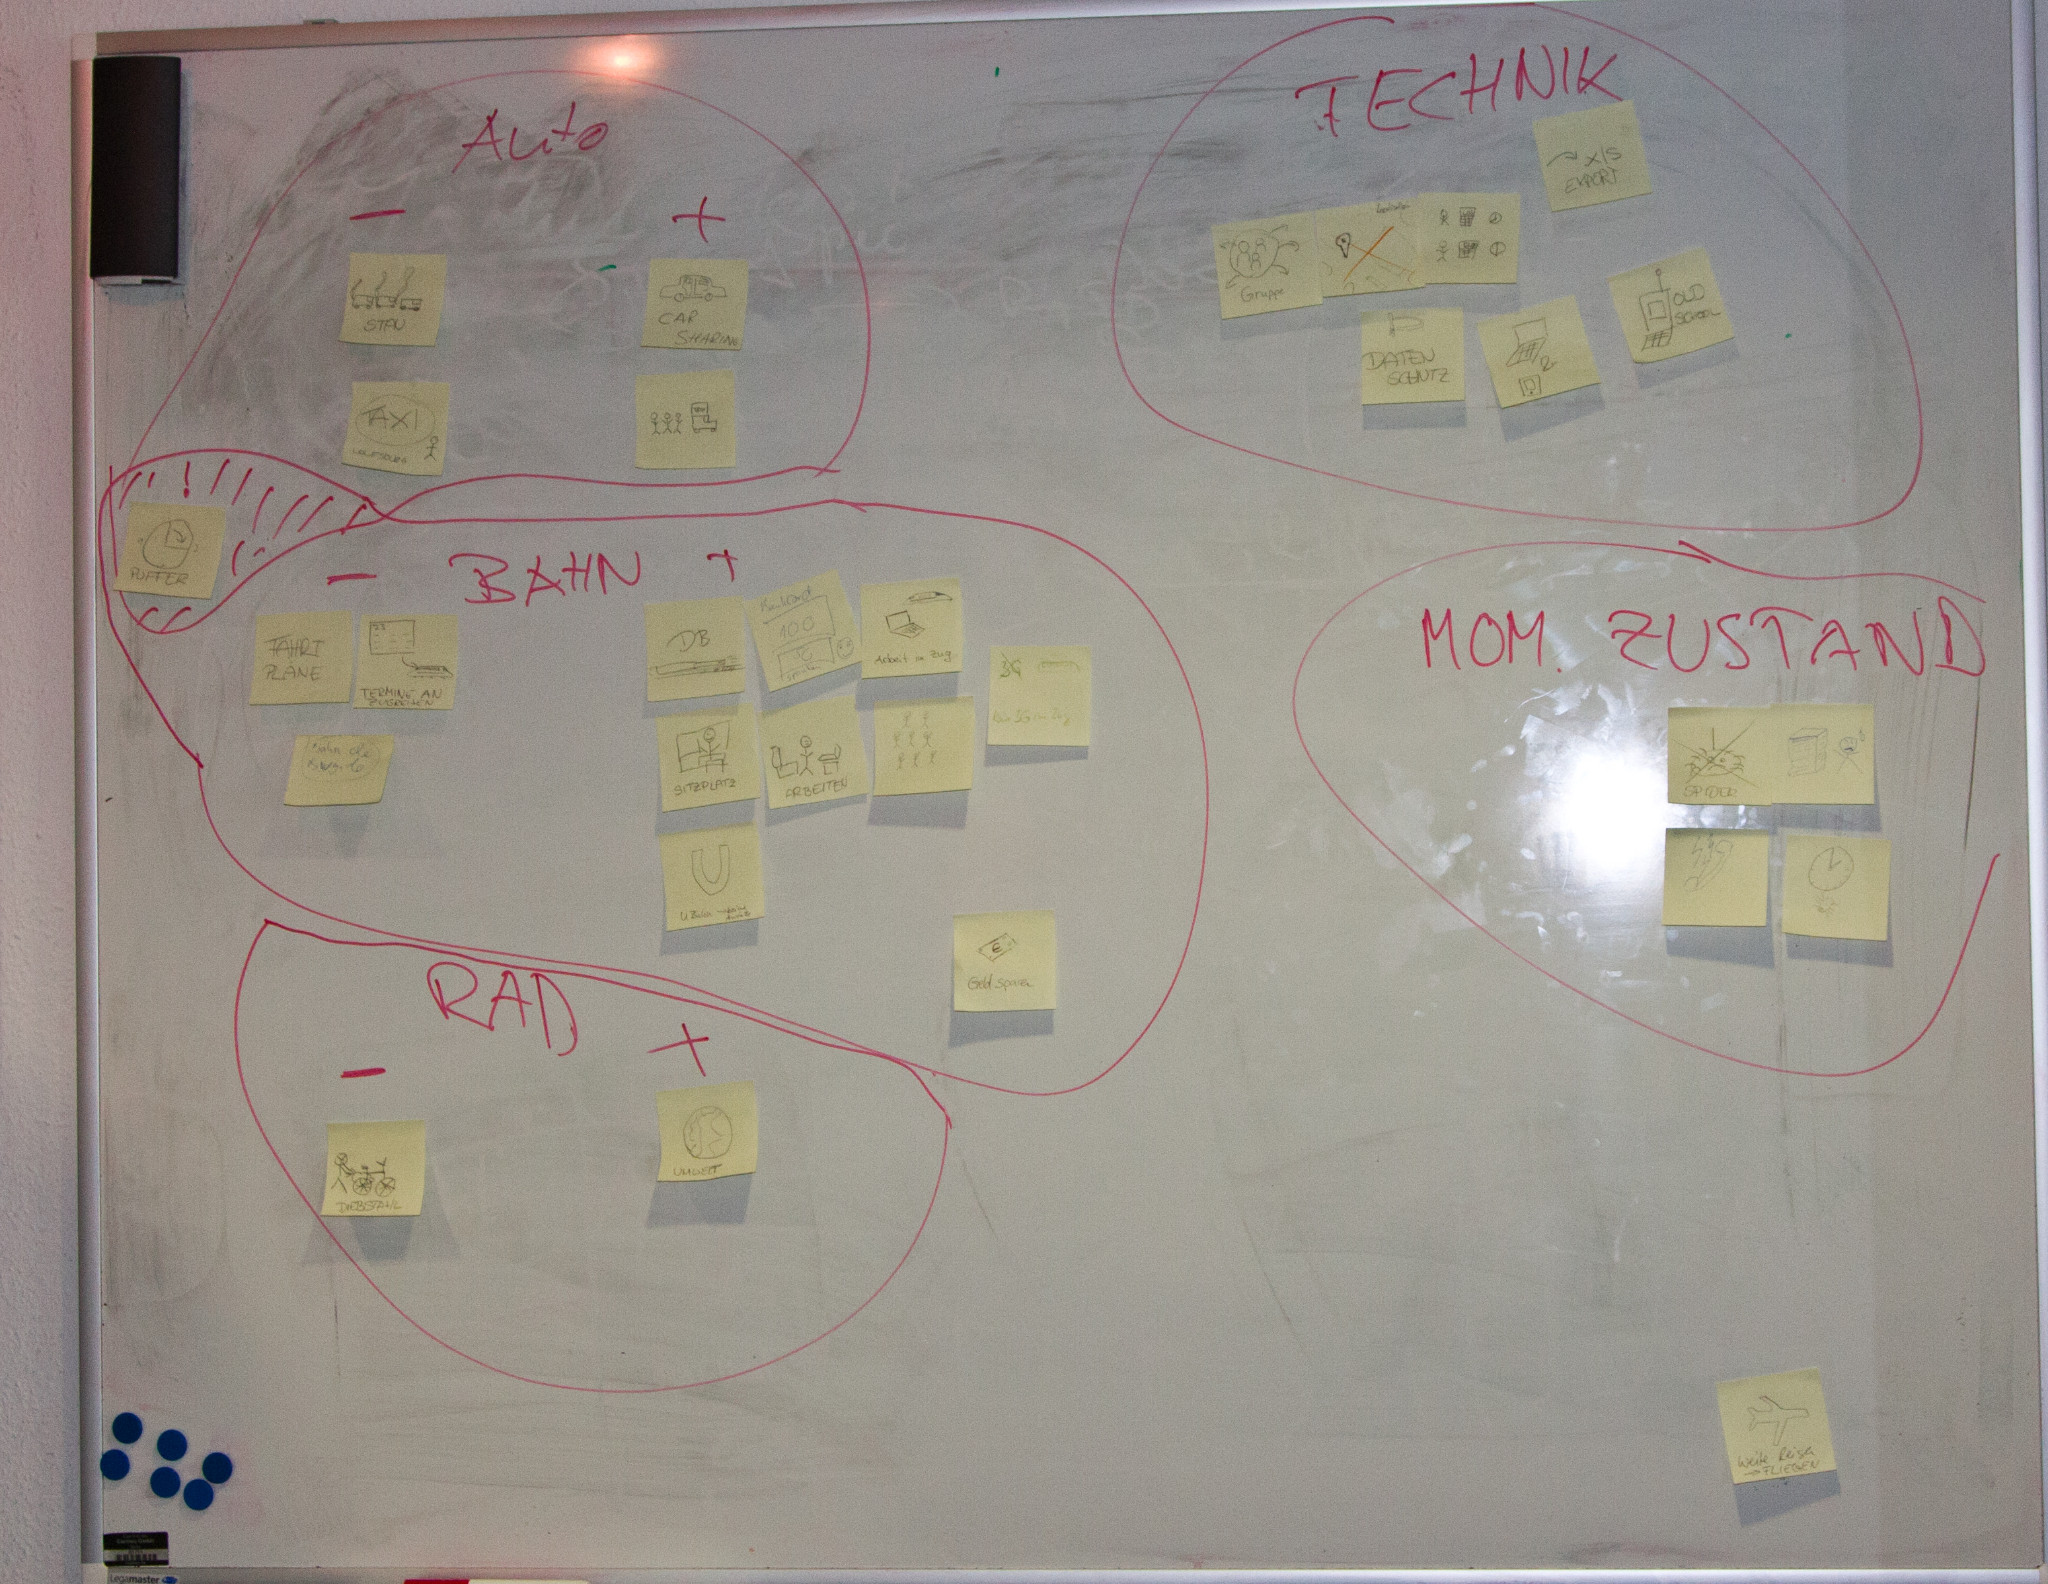
\includegraphics[width=\textwidth]{images/mindmap1.jpg}
		\caption{first try of clustering}
		\label{fig:mindmap1}
	\end{subfigure}
	\begin{subfigure}[b]{0.3\textwidth}
		\centering
		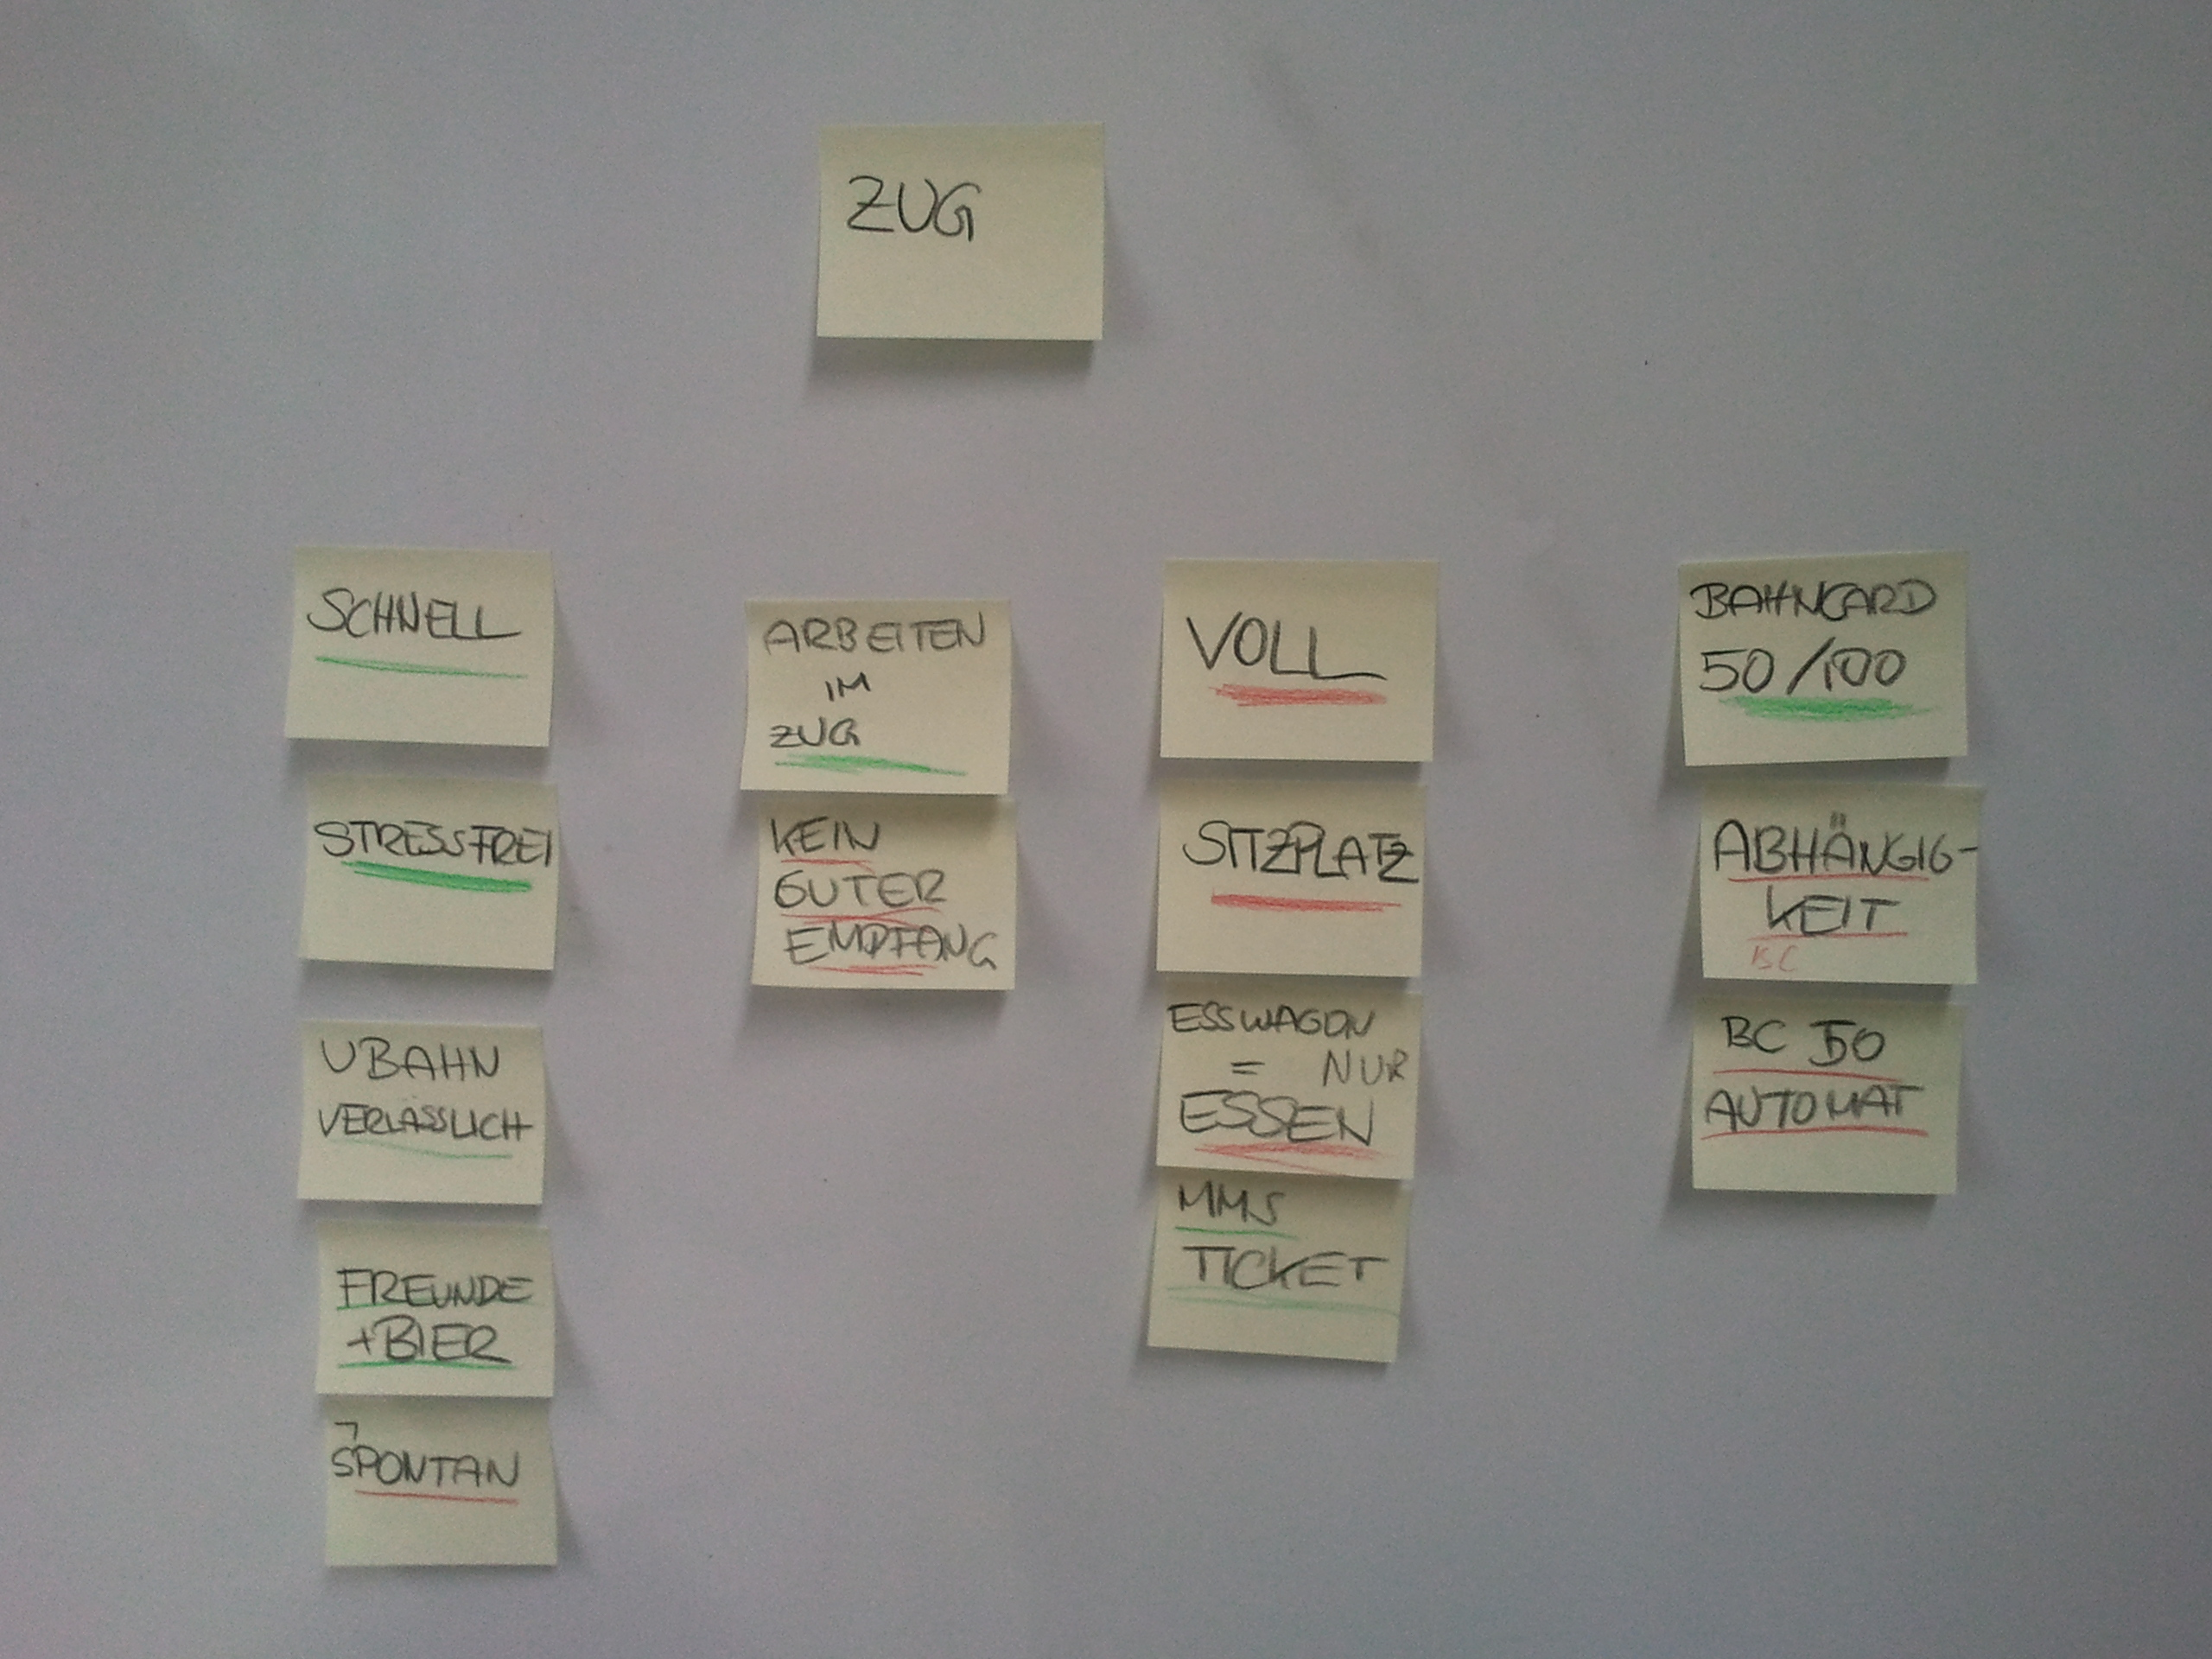
\includegraphics[width=\textwidth]{images/mindmap2.jpg}
		\caption{ cut out 'train'}
		\label{fig:mindmap2}
	\end{subfigure}
	\begin{subfigure}[b]{0.3\textwidth}
		\centering
		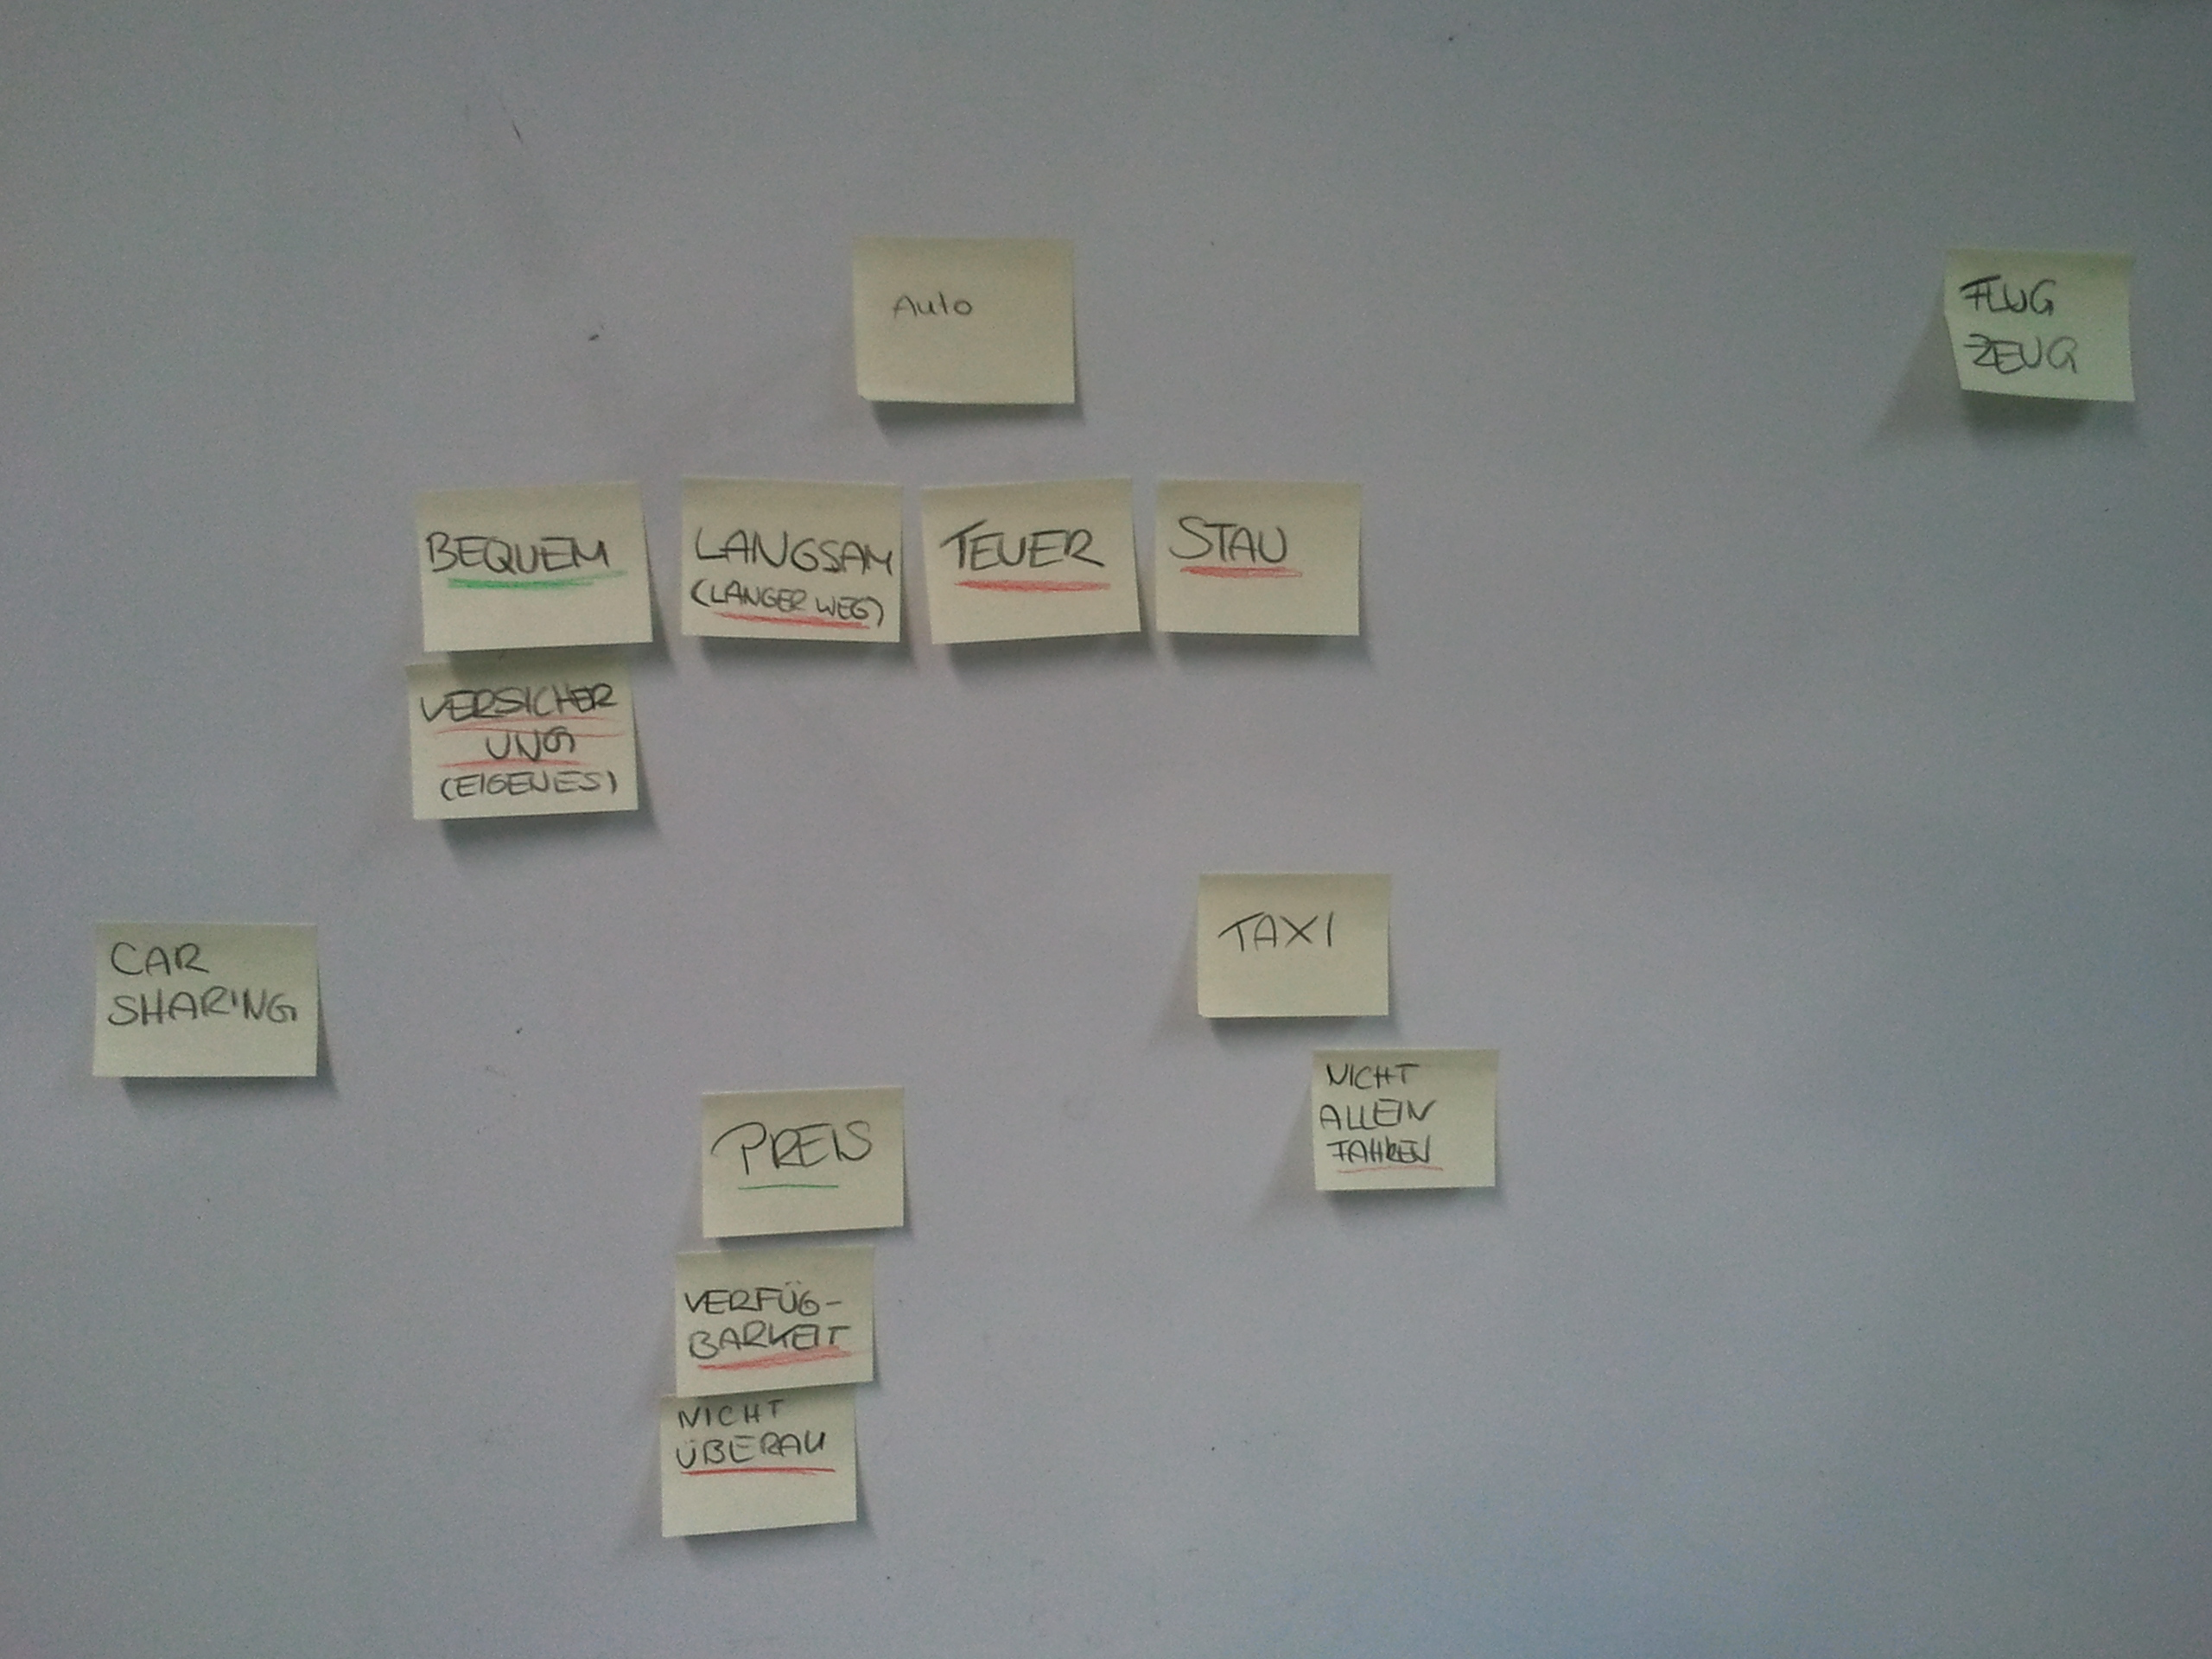
\includegraphics[width=\textwidth]{images/mindmap3.jpg}
		\caption{ cut out 'car'}
		\label{fig:mindmap3}
	\end{subfigure}
	\caption{clustering}
	\label{fig:clustering}
\end{figure}

\section{evaluation}

After the SSC-process it was clear, that every transportation has its own ad- and disadvantages, but their use depends hardy on
whether the person had a bahncard 50 or 100. bahncard 100 people have more problems with reserving seats in the train and
spontaneous traveling whereas bahncard 50 workers have trouble with getting their tickets and finding the right wagon.
bahncard100-people drive more by car, bahncard50 users more by bike or public urban transport.
But both use mainly taxis in Wolfsburg to travel from the main line to their plant and mostly they must disburse a lot of money
for that. 
